% =====================================================================
%  Carga dinámica: balanceo estático vs dinámico (Maestro-Trabajador)
%  Diseño formal (Times, azul marino).   Compilar con XeLaTeX (2 veces):
%      xelatex main.tex
%  (en Overleaf: Menú > Compiler > XeLaTeX)
%  Fuente: Times New Roman si está instalada, si no TeX Gyre Termes ; las figuras en ../resultados/figuras_formal/
%  Guion del expositor:  python guion.py && pdflatex guion.tex
%  Antes: python ../tabla_latex.py   (genera numeros.tex)
% =====================================================================
\documentclass[aspectratio=169,12pt,t]{beamer}

\usepackage{fontspec}
\IfFileExists{spanish.ldf}{\usepackage[spanish,es-noshorthands]{babel}}{\usepackage[english]{babel}}
\usepackage{booktabs,array,colortbl,graphicx,amsmath,listings}
\usepackage{tikz}
\usetikzlibrary{arrows.meta,positioning,calc,patterns,backgrounds,shapes.geometric,decorations.pathreplacing,fit}

% ---------- datos de la portada ----------
\newcommand{\materia}{Cómputo Paralelo Distribuido}
\newcommand{\grupo}{7C}
\newcommand{\carrera}{Ingeniería en Sistemas y Tecnología de la Información}

% Generado por tabla_latex.py - no editar a mano
\newcommand{\tEstHet}{2.41}
\newcommand{\tCicHet}{2.29}
\newcommand{\tPondHet}{0.91}
\newcommand{\tDinUnoHet}{0.84}
\newcommand{\tDinHet}{0.92}
\newcommand{\tGuiHet}{1.05}
\newcommand{\tEstHom}{0.63}
\newcommand{\tDinHom}{0.62}
\newcommand{\tIdealHet}{0.80}
\newcommand{\tUnNodoHet}{2.21}
\newcommand{\tEstDeg}{1.53}
\newcommand{\tCicDeg}{1.24}
\newcommand{\tDinDeg}{0.75}
\newcommand{\tGuiDeg}{0.65}
\newcommand{\spEstHet}{0.92}
\newcommand{\spDinHet}{2.39}
\newcommand{\efDinHet}{87}
\newcommand{\efEstHet}{33}
\newcommand{\utEstHet}{49}
\newcommand{\utDinHet}{91}
\newcommand{\mejoraHet}{2.6}
\newcommand{\mejoraDeg}{2.0}
\newcommand{\chunkMejor}{2}
\newcommand{\tChunkMejor}{0.97}
\newcommand{\chunkPeor}{60}
\newcommand{\tChunkPeor}{2.43}
\newcommand{\spDinOcho}{4.9}
\newcommand{\spEstOcho}{1.9}


% ---------- tipografía: Times New Roman (o TeX Gyre Termes, su equivalente libre) ----------
\IfFontExistsTF{Times New Roman}{\def\fuenteserif{Times New Roman}}{\def\fuenteserif{TeX Gyre Termes}}
\setmainfont{\fuenteserif}
\setsansfont{\fuenteserif}
\setmonofont{Latin Modern Mono}[Scale=0.88]
\newcommand{\kalamL}{}
\usefonttheme{professionalfonts}
\renewcommand{\familydefault}{\sfdefault}

% ---------- paleta: blanco, tinta y azul marino ----------
\definecolor{papel}{HTML}{FFFFFF}
\definecolor{hoja}{HTML}{FFFFFF}
\definecolor{panel}{HTML}{F2F2F2}
\definecolor{tinta}{HTML}{111111}
\definecolor{suave}{HTML}{555555}
\definecolor{regla}{HTML}{CCCCCC}
\definecolor{trazo}{HTML}{999999}
\definecolor{estatico}{HTML}{9B2335}
\definecolor{dinamico}{HTML}{1F3A68}
\definecolor{guiado}{HTML}{2E7D7A}
\definecolor{ocre}{HTML}{B8860B}

\setbeamercolor{background canvas}{bg=papel}
\setbeamercolor{normal text}{fg=tinta}
\setbeamersize{text margin left=1.2cm,text margin right=1.2cm}
\setbeamertemplate{navigation symbols}{}
\setbeamertemplate{itemize item}{\color{dinamico}\textbullet}
\setbeamertemplate{itemize subitem}{\color{estatico}\textbullet}
\setlength{\leftmargini}{1.1em}

% ---------- bloques (block, alertblock, exampleblock): plano, gris claro ----------
\setbeamertemplate{blocks}[default]
\setbeamerfont{block title}{size=\small,series=\bfseries}
\setbeamerfont{block body}{size=\small}
\setbeamercolor{block title}{fg=dinamico,bg=panel}
\setbeamercolor{block body}{fg=tinta,bg=panel}
\setbeamercolor{block title alerted}{fg=estatico,bg=panel}
\setbeamercolor{block body alerted}{fg=tinta,bg=panel}
\setbeamercolor{block title example}{fg=guiado,bg=panel}
\setbeamercolor{block body example}{fg=tinta,bg=panel}

% ---------- encabezado y pie ----------
\newcommand{\dos}[1]{\ifnum#1<10 0\fi#1}
\setbeamertemplate{frametitle}{%
  \vskip 3ex
  {\fontsize{22}{25}\selectfont\color{dinamico}\insertframetitle\par}
  \vskip 0.8ex
  {\color{regla}\hrule height .5pt}\vskip -0.2cm}
\setbeamertemplate{footline}{%
  \leavevmode\hbox to \paperwidth{\hspace*{1.2cm}%
    {\fontsize{8}{9}\selectfont\color{suave}Carga dinámica \hfill \insertframenumber\,/\,\inserttotalframenumber}\hspace*{1.2cm}}\vskip 2.4ex}

% ---------- macros de texto ----------
\newcommand{\ok}[1]{\leavevmode{\color{dinamico}#1}}
\newcommand{\ko}[1]{\leavevmode{\color{estatico}#1}}
\newcommand{\mono}[1]{\leavevmode{\ttfamily\color{guiado}#1}}
\newcommand{\fuente}[1]{\vfill{\fontsize{8.5}{10}\selectfont\color{suave}#1}}
\newcommand{\etq}[2]{{\fontsize{9}{11}\selectfont\addfontfeature{LetterSpace=10}\color{#1}\MakeUppercase{#2}}}
\newcommand{\numeral}[2]{{\kalamL\fontsize{30}{32}\selectfont\color{#1}#2}}
\newcommand{\grande}[2]{{\kalamL\fontsize{30}{32}\selectfont\color{#1}#2}}
\renewcommand{\arraystretch}{1.3}
\setlength{\aboverulesep}{1.2pt}\setlength{\belowrulesep}{1.2pt}\urlstyle{same}
\newcommand{\mx}{\mathop{\text{máx}}\limits}
\newcommand{\linea}{{\color{regla}\rule{\linewidth}{.5pt}}}

% ---------- estilos de TikZ ----------
\tikzset{
  nodo/.style={rounded corners=2pt,fill=hoja,draw=trazo,line width=.5pt,
    inner sep=4pt,text=tinta,font=\small,align=center},
  flecha/.style={-{Stealth[length=4.5pt]},line width=.8pt,color=suave},
  txtp/.style={font=\scriptsize,text=suave},
  txtm/.style={font=\ttfamily\scriptsize,text=guiado},
  ocioso/.style={pattern=north east lines,pattern color=trazo},
}

% ---------- dibujos: persona (con gorro opcional) y caja ----------
\tikzset{pics/persona/.style args={#1/#2}{code={
  \fill[#1] (0,.42) circle (.15);
  \fill[#1] (-.24,0) .. controls (-.24,.3) and (.24,.3) .. (.24,0) -- cycle;
  \ifnum#2=1
    \draw[fill=hoja,draw=tinta,line width=.4pt] (-.12,.55) rectangle (.12,.68);
    \draw[fill=hoja,draw=tinta,line width=.4pt] (0,.72) ellipse (.17 and .09);
  \fi}}}
\newcommand{\caja}[3]{\fill[#3] (#1,#2) rectangle ++(.32,.32);\draw[papel,line width=.5pt] ({#1+.16},#2) -- ++(0,.32);}

% ---------- pseudocódigo ----------
\lstdefinelanguage{pseudo}{morekeywords={PARA,CADA,EN,MIENTRAS,SI,ENTONCES,SINO,
  REPETIR,ENVIAR,RECIBIR,SCATTER,BARRERA,salir},sensitive=true,morecomment=[l]{//}}
\lstset{language=pseudo,
  basicstyle=\ttfamily\fontsize{6.2}{7.2}\selectfont\color{tinta},
  keywordstyle=\color{dinamico}\bfseries,commentstyle=\color{suave},
  backgroundcolor=\color{hoja},frame=single,rulecolor=\color{regla},framesep=4pt,
  xleftmargin=5pt,xrightmargin=2pt,showstringspaces=false,breaklines=true,
  keepspaces=true,columns=fullflexible,aboveskip=2pt,belowskip=0pt,
  literate={<-}{{$\leftarrow$}}1 {->}{{$\rightarrow$}}1}

\begin{document}

% ===================================================================== 1
\begin{frame}[plain]
\begin{tikzpicture}[remember picture,overlay]
  \node[anchor=north,text width=13cm,align=center,inner sep=0] at ([yshift=-.9cm]current page.north) {%
    {\fontsize{9.5}{11.5}\selectfont\addfontfeature{LetterSpace=18}\color{suave}\MakeUppercase{UVP \;·\; \materia}}\\[7pt]
    {\color{regla}\rule{1.6cm}{.6pt}}};
  \node[align=center,inner sep=0,text width=13cm] at ([yshift=-.2cm]current page.center) {%
    {\kalamL\fontsize{42}{46}\selectfont\color{tinta}Carga dinámica}\\[8pt]
    {\fontsize{11}{15}\selectfont\color{suave}Balanceo de carga estático vs.\ dinámico\\en una arquitectura Maestro–Trabajador}\\[11pt]
    {\color{regla}\rule{1.6cm}{.6pt}}\\[8pt]
    {\fontsize{9.5}{11.5}\selectfont\addfontfeature{LetterSpace=18}\color{suave}\MakeUppercase{Alumnos}}\\[4pt]
    {\fontsize{10.5}{14}\selectfont Jared Méndez Valencia \;\color{regla}|\;\color{tinta} Daniel del Valle Andrade\\
     Johan Lezama Núñez \;\color{regla}|\;\color{tinta} Camila Serrano Trinidad}};
  \node[anchor=south,text width=13cm,align=center,inner sep=0,font=\fontsize{9}{11}\selectfont,text=suave] at ([yshift=.45cm]current page.south) {\carrera\\Grupo \grupo};
\end{tikzpicture}
\note[item]{Presentación del equipo: cada integrante dice su nombre y qué parte expone.}
\note[item]{Frase gancho: ``¿Qué pasa cuando un nodo lento frena a uno rápido?'' Hoy lo vemos con teoría y con una simulación en una laptop.}
\end{frame}

% ===================================================================== 2
\section{Introducción}
\begin{frame}{Objetivos}
{\kalamL\fontsize{15}{20}\selectfont Comprender y comparar el balanceo de carga \textbf{\color{estatico}estático} y \textbf{\color{dinamico}dinámico} en una arquitectura Maestro–Trabajador, y demostrarlo con una simulación en MPI.\par}
\vspace{.55cm}
\begin{columns}[T,onlytextwidth]
\column{.22\textwidth}\linea\\[3pt]\numeral{dinamico}{01}\\[2pt]\textbf{Explicar}\\[2pt]{\small\color{suave}Cómo se reparte el trabajo para que un nodo lento no frene a uno rápido.}
\column{.22\textwidth}\linea\\[3pt]\numeral{dinamico}{02}\\[2pt]\textbf{Comparar}\\[2pt]{\small\color{suave}El algoritmo estático vs.\ el dinámico, con paquetes según la velocidad.}
\column{.22\textwidth}\linea\\[3pt]\numeral{dinamico}{03}\\[2pt]\textbf{Proponer}\\[2pt]{\small\color{suave}Estrategias para evitar nodos en espera.}
\column{.22\textwidth}\linea\\[3pt]\numeral{dinamico}{04}\\[2pt]\textbf{Medir}\\[2pt]{\small\color{suave}Tiempo, speedup, eficiencia y ocio con Python y mpi4py.}
\end{columns}
\note[item]{Los cuatro objetivos específicos coinciden con lo que pide el tema: cómo se reparte, algoritmo estático vs dinámico, paquetes según velocidad y estrategias para evitar nodos en espera.}
\end{frame}

% ===================================================================== 3
\section{El problema}
\begin{frame}{Un nodo lento frena a uno rápido}
\begin{columns}[c,onlytextwidth]
\column{.66\textwidth}
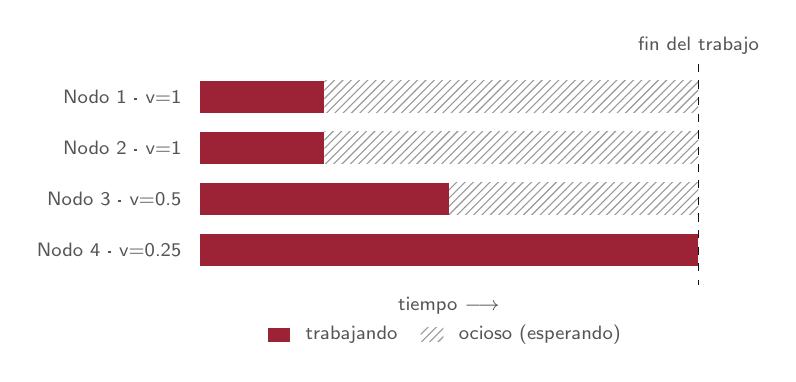
\begin{tikzpicture}[scale=.72]
  \foreach \i/\d/\n in {0/2.2/{Nodo 1 · v=1},1/2.2/{Nodo 2 · v=1},2/4.4/{Nodo 3 · v=0.5},3/8.8/{Nodo 4 · v=0.25}}{
    \node[txtp,anchor=east] at (-.15,{-\i*.9-.28}) {\n};
    \fill[estatico] (0,{-\i*.9}) rectangle ({\d},{-\i*.9-.56});
    \fill[ocioso] ({\d},{-\i*.9}) rectangle (8.8,{-\i*.9-.56});
  }
  \draw[dashed,tinta,line width=.6pt] (8.8,.3) -- (8.8,-3.6);
  \node[txtp,anchor=south] at (8.8,.3) {fin del trabajo};
  \node[txtp,anchor=north] at (4.4,-3.65) {tiempo $\longrightarrow$};
  \fill[estatico] (1.2,-4.6) rectangle ++(.4,.25); \node[txtp,anchor=west] at (1.7,-4.48) {trabajando};
  \fill[ocioso] (3.9,-4.6) rectangle ++(.4,.25); \node[txtp,anchor=west] at (4.4,-4.48) {ocioso (esperando)};
\end{tikzpicture}
\column{.3\textwidth}
\linea\\[4pt]
{\etq{suave}{Reparto igual para todos}}\\[6pt]
{\kalamL\fontsize{24}{26}\selectfont\color{estatico}$T=\mx_i T_i$}\\[6pt]
{\small El trabajo termina cuando termina el \ko{más lento}; los rápidos esperan.}
\end{columns}
\note[item]{Aquí está la idea central de todo el tema: con un reparto igual, el trabajo termina cuando termina el nodo más lento.}
\note[item]{Los nodos rápidos quedan ociosos: se paga hardware que no se aprovecha.}
\end{frame}

\begin{frame}{Conceptos y métricas}
\begin{columns}[T,onlytextwidth]
\column{.47\textwidth}
\small\renewcommand{\arraystretch}{1.05}\arrayrulecolor{regla}
\begin{tabular}{@{}>{\bfseries\color{estatico}}l@{\hspace{.25cm}}l@{}}
Nodo & máquina o proceso MPI\\[2pt] \midrule[.4pt]
Tarea & unidad de trabajo con costo\\[2pt] \midrule[.4pt]
Paquete & tareas entregadas juntas\\[2pt] \midrule[.4pt]
Maestro & reparte y coordina\\[2pt] \midrule[.4pt]
Trabajador & ejecuta y pide más\\[2pt] \midrule[.4pt]
Heterogeneidad & velocidades $v_i$ distintas
\end{tabular}
\column{.03\textwidth}\column{.46\textwidth}
\renewcommand{\arraystretch}{1}
\begin{tabular}{@{}l@{\hspace{.6cm}}l@{}}
\etq{suave}{Tiempo total} & \large $T=\mx_i T_i$\\[7pt]\midrule[.4pt]
\etq{suave}{Speedup} & \large $S=T_{1\,\text{nodo}}/T$\\[7pt]\midrule[.4pt]
\etq{suave}{Eficiencia} & \large $E=T_{\text{ideal}}/T$\\[7pt]\midrule[.4pt]
\etq{suave}{Utilización} & \large $U=\text{ocupado}/T$
\end{tabular}
\end{columns}
\vspace{-2pt}
\begin{block}{Balance ideal}
$T_{\text{ideal}}=\sum_j c_j\big/\sum_i v_i$ \quad (todos terminan a la vez y no hay costo de comunicación)
\end{block}
\note[item]{Define con tus palabras cada concepto; son el vocabulario del resto de la exposición.}
\note[item]{El ideal es el balance perfecto sin costos de comunicación: el trabajo total entre la suma de velocidades. Si la eficiencia es 100\,\% nadie espera.}
\note[item]{Vocabulario de sistemas distribuidos que se usará: heterogeneidad (nodos con velocidades distintas), granularidad (tamaño del paquete), overhead de comunicación (mensajes que no son cómputo), cuello de botella (el maestro o el nodo más lento) y escalabilidad (cómo mejora el tiempo al agregar nodos).}
\note[item]{Referencia de métricas: Pacheco \& Malensek (2022).}
\end{frame}

% ===================================================================== 5
\section{Maestro–Trabajador}
\begin{frame}{Arquitectura Maestro–Trabajador}
\centering
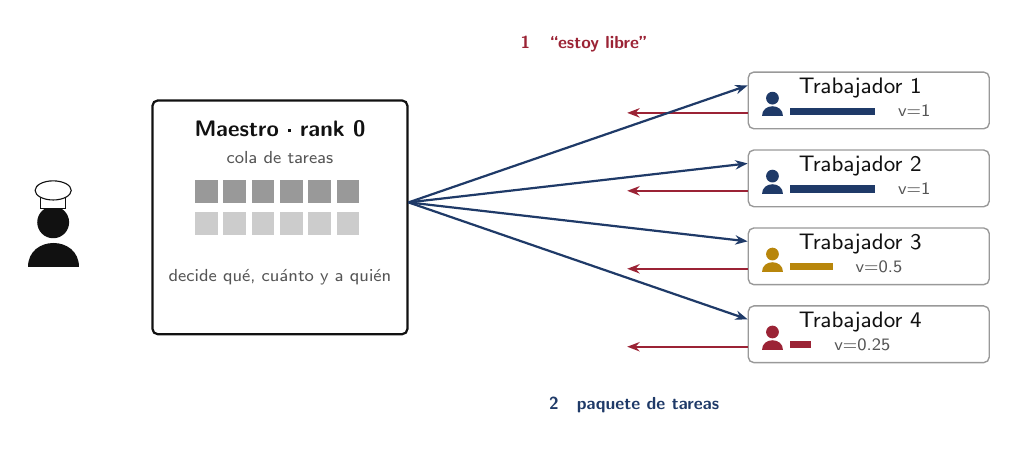
\begin{tikzpicture}[scale=.9,transform shape]
  \node[nodo,minimum width=3.6cm,minimum height=3.3cm,draw=tinta,line width=.8pt] (m) at (0,0) {};
  \pic[scale=1.5] at (-3.2,-.7) {persona={tinta/1}};
  \node[font=\bfseries\small,text=tinta] at (0,1.25) {Maestro · rank 0};
  \node[txtp] at (0,.85) {cola de tareas};
  \foreach \k in {0,...,5}{\fill[trazo] ({-1.2+\k*.4},.2) rectangle ++(.32,.32);}
  \foreach \k in {0,...,5}{\fill[regla] ({-1.2+\k*.4},-.25) rectangle ++(.32,.32);}
  \node[txtp] at (0,-.85) {decide qué, cuánto y a quién};
  \foreach \i/\n/\v/\c in {0/{Trabajador 1}/1/dinamico, 1/{Trabajador 2}/1/dinamico, 2/{Trabajador 3}/0.5/ocre, 3/{Trabajador 4}/0.25/estatico}{
    \node[nodo,minimum width=3.4cm,minimum height=.8cm,anchor=west] (w\i) at (6.6,{1.65-\i*1.1}) {};
    \node[font=\small,text=tinta,anchor=west] at (7.2,{1.82-\i*1.1}) {\n};
    \pic[scale=.6] at (6.95,{1.43-\i*1.1}) {persona={\c/0}};
    \fill[\c] (7.2,{1.45-\i*1.1}) rectangle ({7.2+1.2*\v},{1.45-\i*1.1+.1});
    \node[txtp,anchor=west] at ({7.4+1.2*\v},{1.5-\i*1.1}) {v=\v};
  }
  \foreach \i in {0,...,3}{
    \draw[flecha,estatico] ([yshift=-5pt]w\i.west) -- ++(-1.7,0);
    \draw[flecha,dinamico] ([yshift=6pt]m.east) -- ([yshift=6pt]w\i.west);
  }
  \node[font=\scriptsize\bfseries,text=estatico] at (4.3,2.45) {1 \; ``estoy libre''};
  \node[font=\scriptsize\bfseries,text=dinamico] at (5.0,-2.65) {2 \; paquete de tareas};
\end{tikzpicture}
\fuente{El maestro solo coordina; el que se desocupa pide más trabajo (esquema bajo demanda; Fernandes et al., 2024).}
\note[item]{El maestro (rank 0) tiene la cola de tareas y no calcula. Los trabajadores son los nodos, cada uno con su velocidad.}
\note[item]{Dos mensajes: el trabajador dice ``estoy libre'' y el maestro responde con un paquete.}
\end{frame}

% ===================================================================== 6
\begin{frame}{Protocolo de mensajes}
\centering
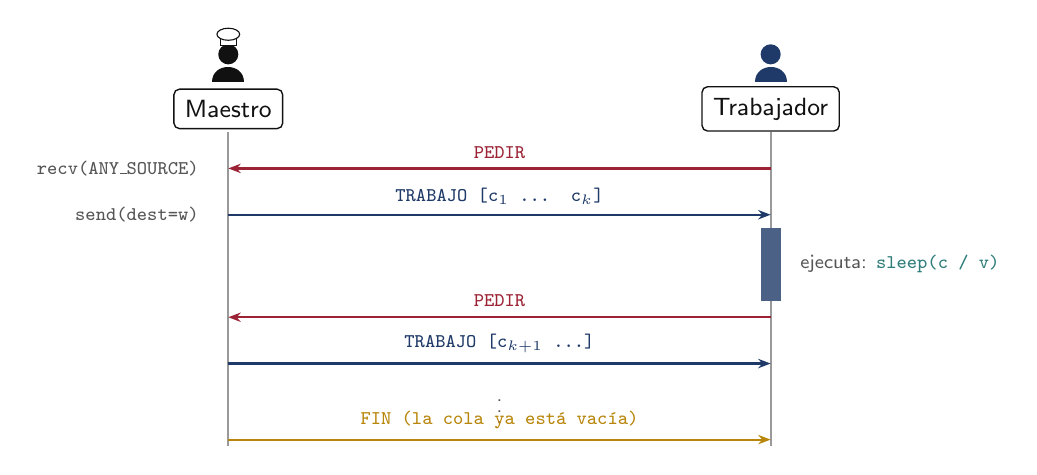
\begin{tikzpicture}[x=1cm,y=1cm,scale=.84]
  \node[nodo,draw=tinta] (M) at (1.2,0) {Maestro};
  \node[nodo,draw=tinta] (T) at (9.4,0) {Trabajador};
  \pic[scale=.85] at (1.2,.4) {persona={tinta/1}};
  \pic[scale=.85] at (9.4,.4) {persona={dinamico/0}};
  \draw[trazo,line width=.7pt] (1.2,-.35) -- (1.2,-5.1);
  \draw[trazo,line width=.7pt] (9.4,-.35) -- (9.4,-5.1);
  \draw[flecha,estatico] (9.4,-.9) -- (1.2,-.9) node[midway,above,txtm,text=estatico] {PEDIR};
  \draw[flecha,dinamico] (1.2,-1.6) -- (9.4,-1.6) node[midway,above,txtm,text=dinamico] {TRABAJO [c$_1$ … c$_k$]};
  \fill[dinamico!80] (9.25,-1.8) rectangle (9.55,-2.9);
  \node[txtp,anchor=west] at (9.7,-2.35) {ejecuta: \mono{sleep(c / v)}};
  \draw[flecha,estatico] (9.4,-3.15) -- (1.2,-3.15) node[midway,above,txtm,text=estatico] {PEDIR};
  \draw[flecha,dinamico] (1.2,-3.85) -- (9.4,-3.85) node[midway,above,txtm,text=dinamico] {TRABAJO [c$_{k+1}$ …]};
  \node[txtp] at (5.3,-4.45) {$\vdots$};
  \draw[flecha,ocre] (1.2,-5.0) -- (9.4,-5.0) node[midway,above,txtm,text=ocre] {FIN (la cola ya está vacía)};
  \node[txtm,anchor=east,text=suave] at (.9,-.9) {recv(ANY\_SOURCE)};
  \node[txtm,anchor=east,text=suave] at (.9,-1.6) {send(dest=w)};
\end{tikzpicture}
\note[item]{Tres tipos de mensaje: PEDIR, TRABAJO y FIN. En mpi4py el maestro usa recv con ANY\_SOURCE para atender al primero que pida.}
\note[item]{El trabajador es quien manda el ritmo: pide cuando termina. Eso es lo que hace al esquema dinámico.}
\end{frame}

% ===================================================================== 7
\section{Estático vs. dinámico}
\begin{frame}{Estático vs.\ dinámico}
\begin{columns}[T,onlytextwidth]
\column{.47\textwidth}
{\etq{estatico}{Estático}} \hfill {\fontsize{9.5}{11.5}\selectfont\color{suave}se decide antes de ejecutar}\\[2pt]\linea\\[8pt]
\centering
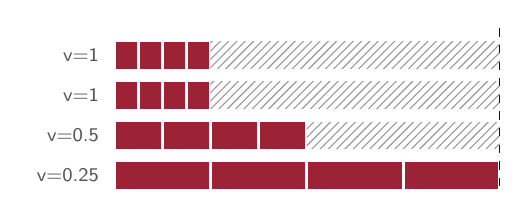
\begin{tikzpicture}[scale=.68]
  \foreach \i/\n/\w in {0/{v=1}/.45,1/{v=1}/.45,2/{v=0.5}/.9,3/{v=0.25}/1.8}{
    \node[txtp,anchor=east] at (-.1,{-\i*.75-.25}) {\n};
    \foreach \k in {1,...,4}{\fill[estatico] ({(\k-1)*\w+.03},{-\i*.75}) rectangle ({\k*\w-.03},{-\i*.75-.5});}
    \pgfmathsetmacro{\fin}{4*\w}
    \fill[ocioso] ({\fin},{-\i*.75}) rectangle (7.2,{-\i*.75-.5});
  }
  \draw[dashed,tinta,line width=.5pt] (7.2,.25) -- (7.2,-2.8);
\end{tikzpicture}\\[4pt]
{\small Las mismas 4 tareas para todos: el rápido \ko{espera}.}\\[2pt]
{\fontsize{9.5}{11.5}\selectfont\color{suave}1 mensaje por nodo (\mono{Scatter})}
\column{.02\textwidth}
\column{.47\textwidth}
{\etq{dinamico}{Dinámico}} \hfill {\fontsize{9.5}{11.5}\selectfont\color{suave}pide el que se desocupa}\\[2pt]\linea\\[8pt]
\centering
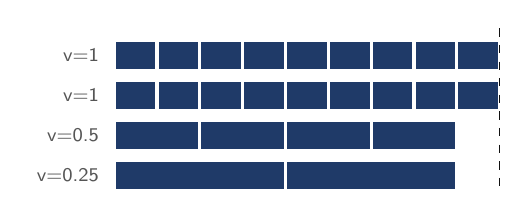
\begin{tikzpicture}[scale=.68]
  \foreach \i/\n/\w/\c in {0/{v=1}/.8/9,1/{v=1}/.8/9,2/{v=0.5}/1.6/4,3/{v=0.25}/3.2/2}{
    \node[txtp,anchor=east] at (-.1,{-\i*.75-.25}) {\n};
    \foreach \k in {1,...,9}{\ifnum\k>\c\relax\else
      \fill[dinamico] ({(\k-1)*\w+.03},{-\i*.75}) rectangle ({\k*\w-.03},{-\i*.75-.5});\fi}
  }
  \draw[dashed,tinta,line width=.5pt] (7.2,.25) -- (7.2,-2.8);
\end{tikzpicture}\\[4pt]
{\small Paquetes iguales: el rápido hace \ok{más} y todos terminan juntos.}\\[2pt]
{\fontsize{9.5}{11.5}\selectfont\color{suave}cola en el maestro · $\approx 2$ mensajes por paquete}
\end{columns}
\note[item]{Izquierda, estático: el maestro decide todo al inicio. Con el mismo número de tareas para todos, el nodo rápido termina antes y espera (zona rayada).}
\note[item]{Derecha, dinámico: con paquetes iguales el nodo rápido pide más veces y hace más tareas; todos terminan casi juntos. El costo es la comunicación.}
\end{frame}

% ===================================================================== 8
\begin{frame}[fragile]{Algoritmos: estático y dinámico}
\lstset{basicstyle=\ttfamily\fontsize{7.4}{8.8}\selectfont\color{tinta}}
\begin{columns}[T,onlytextwidth]
\column{.45\textwidth}
{\etq{estatico}{Estático}}\\[3pt]
\begin{lstlisting}
// MAESTRO
repartir las tareas entre los nodos
ENVIAR a cada nodo su lote

// NODO
lote <- RECIBIR
ejecutar todas sus tareas
BARRERA      // espera al más lento
\end{lstlisting}\vspace{12pt}
{\small\color{suave}En el estático el maestro decide todo al inicio; en el dinámico, \textbf{el nodo que termina pide más}.}
\column{.53\textwidth}
{\etq{dinamico}{Dinámico}}\\[3pt]
\begin{lstlisting}
// MAESTRO
cola <- todas las tareas
MIENTRAS haya nodos activos:
    i <- RECIBIR(cualquiera)
    SI cola no vacía ENTONCES
        ENVIAR(i, paquete)
    SINO
        ENVIAR(i, FIN)

// NODO
REPETIR
    ENVIAR(PEDIR)
    paquete <- RECIBIR
    SI paquete = FIN ENTONCES salir
    ejecutar el paquete
\end{lstlisting}
\end{columns}
\note[item]{Estático: el maestro arma los lotes, los envía con un Scatter y cada trabajador procesa lo suyo; la barrera final es la espera.}
\note[item]{Dinámico: el maestro atiende el primer PEDIR que llegue y responde con un paquete; termina cuando la cola se vacía y envía FIN. El código real está en el archivo aparte balanceo.py.}
\end{frame}

% ===================================================================== (nueva) diagrama de flujo
\begin{frame}{Diagrama de flujo del maestro dinámico}
\begin{columns}[c,onlytextwidth]
\column{.68\textwidth}
\centering
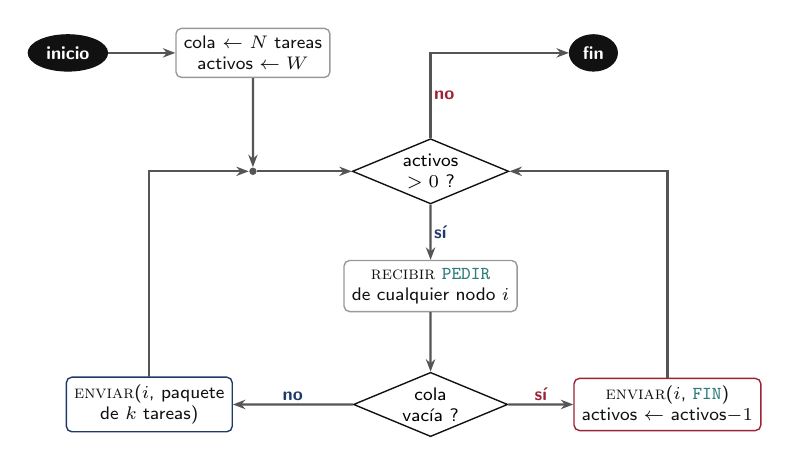
\begin{tikzpicture}[scale=.94,transform shape,
  dec/.style={diamond,aspect=2.4,draw=tinta,fill=hoja,line width=.5pt,inner sep=1pt,font=\scriptsize,align=center},
  proc/.style={nodo,font=\scriptsize,inner sep=3pt},
  term/.style={ellipse,draw=tinta,fill=tinta,text=papel,font=\scriptsize\bfseries,inner sep=2.5pt},
  et/.style={font=\scriptsize\bfseries,inner sep=1pt}]
  \node[term] (ini) at (0,1.6) {inicio};
  \node[proc] (init) at (2.5,1.6) {cola $\leftarrow$ $N$ tareas\\ activos $\leftarrow W$};
  \node[circle,fill=suave,inner sep=1pt] (j) at (2.5,0) {};
  \node[dec] (d1) at (4.9,0) {activos\\$>0$ ?};
  \node[term] (fin) at (7.1,1.6) {fin};
  \node[proc] (rec) at (4.9,-1.55) {\textsc{recibir} \mono{PEDIR}\\de cualquier nodo $i$};
  \node[dec] (d2) at (4.9,-3.15) {cola\\vacía ?};
  \node[proc,draw=dinamico] (e1) at (1.1,-3.15) {\textsc{enviar}($i$, paquete\\de $k$ tareas)};
  \node[proc,draw=estatico] (e2) at (8.1,-3.15) {\textsc{enviar}($i$, \mono{FIN})\\activos $\leftarrow$ activos$-1$};
  \draw[flecha] (ini) -- (init);
  \draw[flecha] (init) -- (j);
  \draw[flecha] (j) -- (d1);
  \draw[flecha] (d1.north) |- (fin.west) node[et,pos=.25,right,text=estatico] {no};
  \draw[flecha] (d1) -- (rec) node[et,midway,right,text=dinamico] {sí};
  \draw[flecha] (rec) -- (d2);
  \draw[flecha] (d2) -- (e1) node[et,midway,above,text=dinamico] {no};
  \draw[flecha] (d2) -- (e2) node[et,midway,above,text=estatico] {sí};
  \draw[flecha] (e1.north) |- (j);
  \draw[flecha] (e2.north) |- (d1.east);
\end{tikzpicture}
\column{.3\textwidth}
\begin{block}{Invariantes}
Cada tarea sale de la cola \textbf{una sola vez}. El ciclo termina cuando \mono{activos}\,$=0$.
\end{block}
\vspace{2pt}
\begin{exampleblock}{Mensajes}
$M=2\big(\lceil N/k\rceil+W\big)$
\end{exampleblock}
\end{columns}
\note[item]{Este es el diagrama de flujo del maestro. Se lee de arriba hacia abajo: se inicializa la cola con las N tareas y el contador de trabajadores activos con W. Mientras haya trabajadores activos, el maestro se bloquea en una recepción con ANY\_SOURCE y atiende al primero que pida.}
\note[item]{Si todavía hay tareas, responde con un paquete de k tareas; si la cola ya está vacía, responde FIN y descuenta un trabajador activo. Cuando activos llega a cero, el maestro termina.}
\note[item]{Invariante de corrección: cada tarea sale de la cola una sola vez, así que no se repite ni se pierde trabajo. Además, cada trabajador recibe exactamente un FIN.}
\note[item]{Conteo de mensajes: hay $\lceil N/k\rceil$ paquetes más un PEDIR final por trabajador; cada PEDIR tiene su respuesta, por eso $M=2(\lceil N/k\rceil+W)$. Con $N=240$, $k=8$ y $W=4$ son 68 mensajes; con $k=4$ serían 128. Esto es el overhead de comunicación que crece cuando k disminuye.}
\end{frame}

\begin{frame}{Cuadro comparativo}
\small\renewcommand{\arraystretch}{1.05}\arrayrulecolor{regla}
\begin{tabular}{@{}>{\bfseries\raggedright\arraybackslash}p{4.4cm}p{4.4cm}>{\raggedright\arraybackslash}p{4.8cm}@{}}
\toprule[.8pt]
\etq{suave}{Criterio} & \etq{estatico}{Estático} & \etq{dinamico}{Dinámico} \\ \midrule[.5pt]
Cuándo se reparte & Antes de ejecutar & Durante la ejecución \\ \midrule[.3pt]
Mensajes & \ok{Pocos (1 por nodo)} & \ko{Muchos ($\approx 2$ por paquete)} \\ \midrule[.3pt]
Nodos distintos o tareas desiguales & \ko{Espera el más rápido} & \ok{Se adapta solo} \\ \midrule[.3pt]
Un nodo que se degrada & \ko{No reacciona} & \ok{Reparte menos a ese nodo} \\ \midrule[.3pt]
Implementación & \ok{Simple} & Más compleja \\ \midrule[.3pt]
Riesgo & Nodos en espera & Maestro como cuello de botella \\
\bottomrule[.8pt]
\end{tabular}
\fuente{Criterios: OpenMP ARB (2021) y Pacheco \& Malensek (2022).}
\note[item]{Este es el cuadro resumen de la comparación. Subraya: estático gana en simplicidad y pocos mensajes; dinámico gana cuando hay heterogeneidad o cargas impredecibles.}
\end{frame}

% ===================================================================== 10
% ===================================================================== 10
\begin{frame}{Paquetes según la velocidad}
\begin{columns}[c,onlytextwidth]
\column{.64\textwidth}
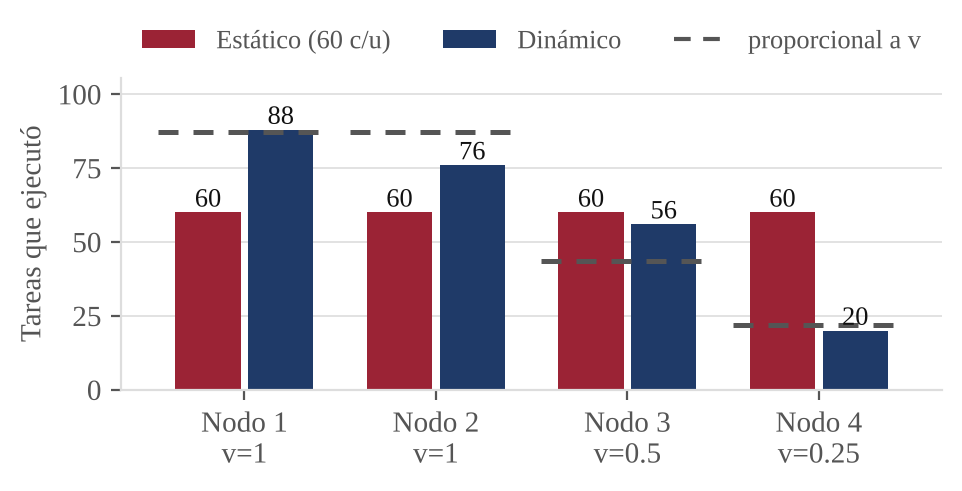
\includegraphics[width=\linewidth,height=4.4cm,keepaspectratio]{../resultados/figuras_formal/tareas_nodo.png}
\column{.33\textwidth}
{\etq{dinamico}{Dinámico}}\\[2pt]\linea\\[4pt]
{\small No se mide la velocidad: el nodo rápido \textbf{pide más veces}.}\\[12pt]
{\etq{guiado}{Guiado}}\\[2pt]\linea\\[4pt]
{\normalsize $k=\mx\!\big(k_{\text{mín}},\lceil \tfrac{\text{restantes}}{f\cdot W}\rceil\big)$}\\[4pt]
{\small Paquetes \textbf{grandes al inicio}, chicos al final.}
\end{columns}
\fuente{Equivale a las planificaciones dynamic y guided de OpenMP (OpenMP ARB, 2021).}
\note[item]{Respuesta a la pregunta del tema: el maestro nunca conoce las velocidades. El nodo rápido termina antes, pide antes y recibe más paquetes. Las líneas punteadas son el reparto ideal proporcional a la velocidad.}
\note[item]{Guiado: los primeros paquetes son grandes (menos mensajes) y se encogen al final para que nadie se quede con un paquete enorme cuando casi no hay trabajo.}
\end{frame}

% ===================================================================== 11
\section{Evitar esperas}
\newcommand{\estrategia}[4]{\linea\\[3pt]{\kalamL\fontsize{20}{22}\selectfont\color{#4}#1}\hspace{.4em}\textbf{#2}\\[2pt]{\small\color{suave}#3}}
\begin{frame}{Estrategias para evitar nodos en espera}
\begin{columns}[T,onlytextwidth]
\column{.31\textwidth}\estrategia{1}{Pedir bajo demanda}{Nadie espera mientras haya cola.}{dinamico}\\[2pt]{\fontsize{9.5}{11.5}\selectfont\ok{En el proyecto}}
\column{.31\textwidth}\estrategia{2}{Paquetes guiados}{Grandes al inicio, chicos al final.}{dinamico}\\[2pt]{\fontsize{9.5}{11.5}\selectfont\ok{En el proyecto}}
\column{.31\textwidth}\estrategia{3}{Ponderar por $v_i$}{Si $v_i$ es conocida y estable.}{dinamico}\\[2pt]{\fontsize{9.5}{11.5}\selectfont\ok{En el proyecto}}
\end{columns}
\vspace{.25cm}
\begin{columns}[T,onlytextwidth]
\column{.31\textwidth}\estrategia{4}{Pesadas primero}{Ordenar de mayor a menor costo (LPT).}{trazo}\\[2pt]{\fontsize{9.5}{11.5}\selectfont\color{suave}Trabajo futuro}
\column{.31\textwidth}\estrategia{5}{Prefetch}{Pedir el siguiente paquete antes de terminar.}{trazo}\\[2pt]{\fontsize{9.5}{11.5}\selectfont\color{suave}Trabajo futuro}
\column{.31\textwidth}\estrategia{6}{Robo de trabajo}{El ocioso roba tareas a otro, sin maestro (Fernandes et al., 2024).}{trazo}\\[2pt]{\fontsize{9.5}{11.5}\selectfont\color{suave}Trabajo futuro}
\end{columns}
\note[item]{Las tres primeras las implementé y las medí. Las otras tres son estrategias de la literatura que quedan como trabajo futuro.}
\note[item]{Prefetch y robo de trabajo se mencionan de nuevo en las conclusiones.}
\end{frame}

% ===================================================================== 12
\section{Simulación}
\begin{frame}{Simulación y diseño experimental}
\begin{columns}[T,onlytextwidth]
\column{.47\textwidth}\centering
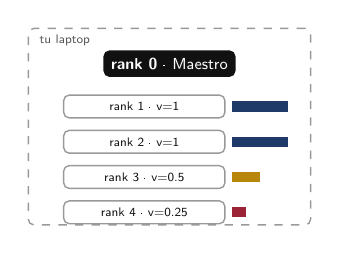
\begin{tikzpicture}[scale=.64,transform shape]
  \node[nodo,minimum width=5.6cm,minimum height=3.9cm,draw=trazo,dashed] at (0,-.05) {};
  \node[txtp,anchor=north west] at (-2.7,1.9) {tu laptop};
  \node[nodo,draw=tinta,fill=tinta,text=papel] at (0,1.2) {\textbf{rank 0} · Maestro};
  \foreach \i/\v/\c/\t in {0/1.0/dinamico/{rank 1 · v=1}, 1/1.0/dinamico/{rank 2 · v=1}, 2/0.5/ocre/{rank 3 · v=0.5}, 3/0.25/estatico/{rank 4 · v=0.25}}{
    \node[nodo,minimum width=3.2cm] at (-.5,{.35-\i*.7}) {\scriptsize \t};
    \fill[\c] (1.25,{.35-\i*.7-.1}) rectangle ++({1.1*\v},.2);
  }
\end{tikzpicture}
\column{.5\textwidth}
\footnotesize\renewcommand{\arraystretch}{1}\arrayrulecolor{regla}
\begin{tabular}{@{}l@{\hspace{.6cm}}l@{}}
\etq{suave}{En la realidad} & \etq{dinamico}{En la simulación}\\[2pt] \midrule[.5pt]
Nodo & proceso MPI\\[1pt] \midrule[.3pt]
Velocidad & factor $v$\\[1pt] \midrule[.3pt]
Cómputo & \mono{sleep(c/v)}\\[1pt] \midrule[.3pt]
Red lenta & \mono{--latencia-ms}\\[1pt] \midrule[.3pt]
Nodo que se degrada & \mono{--degradar}
\end{tabular}
\end{columns}
\vspace{6pt}\linea\\[3pt]
{\etq{suave}{Escenarios medidos}}\\[2pt]
{\small\color{estatico}1\;\color{tinta} nodos iguales \quad\color{estatico}2\;\color{tinta} nodos distintos ($v=1,1,0.5,0.25$) \quad\color{estatico}3\;\color{tinta} tamaño de paquete (1…60)\\
\color{estatico}4\;\color{tinta} 1, 2, 4 y 8 trabajadores \quad\color{estatico}5\;\color{tinta} un nodo que se degrada}\\[3pt]
{\fontsize{8.5}{10}\selectfont\color{suave}240 tareas · costo medio 10\,ms (log-normal) · semilla fija · mediana de 3–5 corridas}
\note[item]{En una laptop todos los procesos son igual de rápidos, entonces simulo la heterogeneidad: cada trabajador tiene un factor de velocidad y tarda costo dividido entre velocidad. Con mpiexec -n 5 hay 1 maestro y 4 trabajadores.}
\note[item]{Usar sleep hace que los resultados no dependan de cuántos núcleos tenga la laptop. También existe un modo real con carga de CPU.}
\note[item]{Cinco escenarios, cada uno con una pregunta: ¿qué pasa con nodos iguales?, ¿con nodos distintos?, ¿cuál es el mejor tamaño de paquete?, ¿cómo escala?, ¿qué pasa si un nodo se degrada? Mismas tareas (semilla fija) para todas las estrategias.}
\end{frame}

% ===================================================================== 13
\section{Resultados}
\begin{frame}{Quién trabaja y quién espera}
\begin{columns}[c,onlytextwidth]
\column{.72\textwidth}
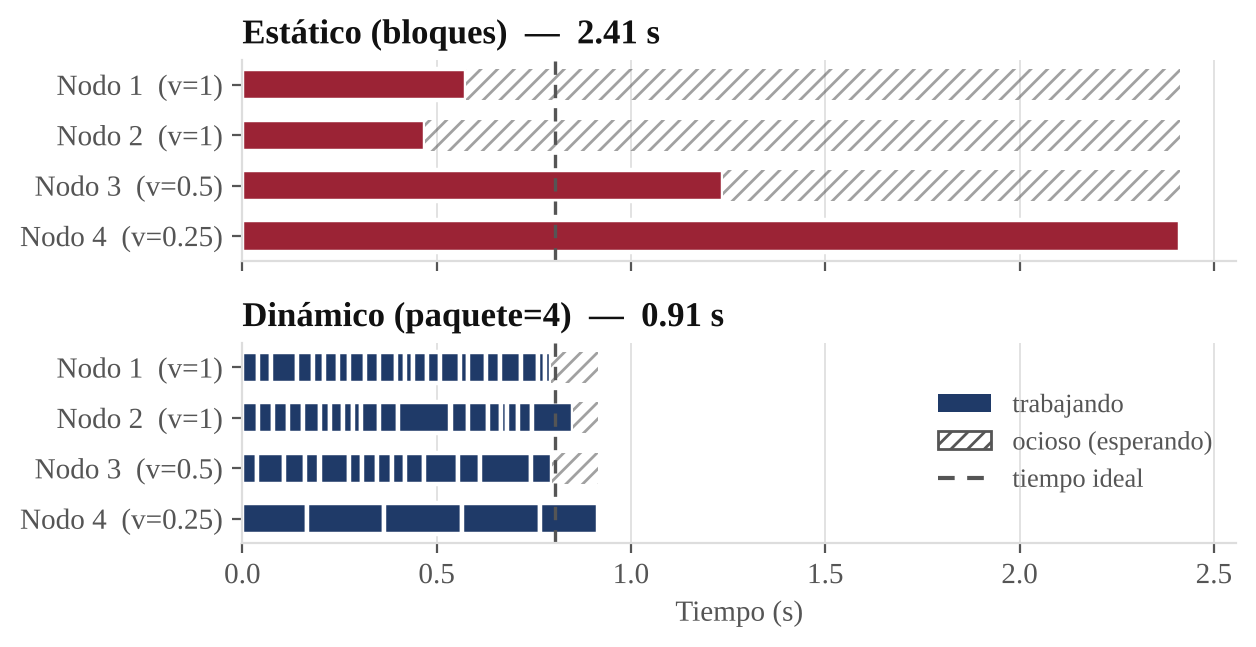
\includegraphics[width=\linewidth,height=5.2cm,keepaspectratio]{../resultados/figuras_formal/gantt.png}
\column{.27\textwidth}
\etq{suave}{Utilización media}\\[2pt]\linea\\[6pt]
\grande{estatico}{\utEstHet\,\%}\\[-2pt]{\fontsize{9.5}{11.5}\selectfont\color{suave}estático}\\[8pt]
\grande{dinamico}{\utDinHet\,\%}\\[-2pt]{\fontsize{9.5}{11.5}\selectfont\color{suave}dinámico}
\end{columns}
\note[item]{Esta es la diapositiva más importante. Arriba, estático: el nodo 4 trabaja todo el tiempo y los demás están rayados, es decir, esperando.}
\note[item]{Abajo, con dinámico, todos terminan casi al mismo tiempo, cerca de la línea punteada de tiempo ideal.}
\end{frame}

% ===================================================================== 14
\begin{frame}{Tiempo total en dos escenarios}
\centering
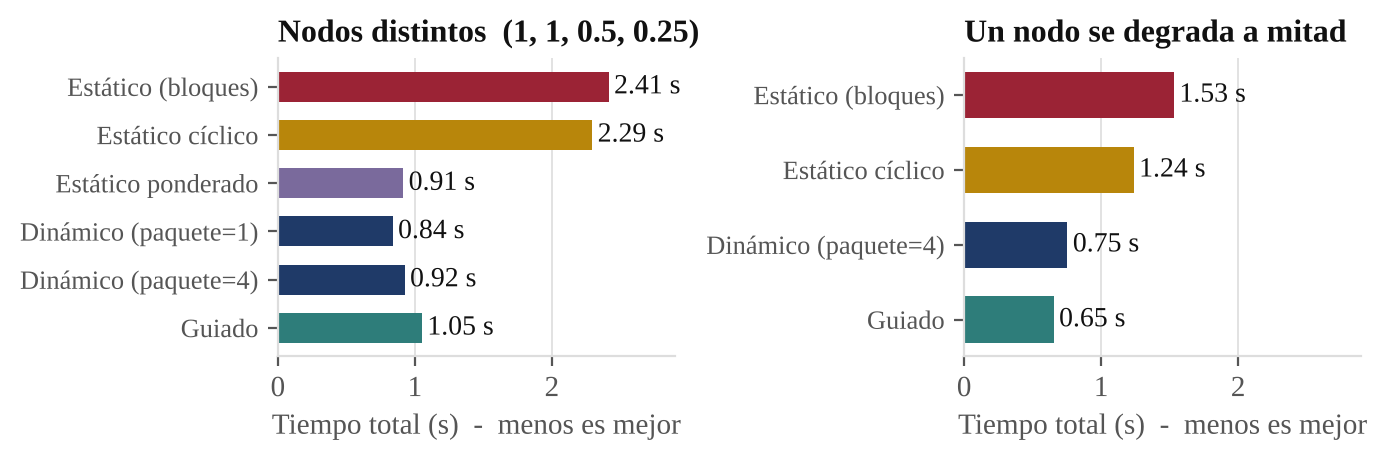
\includegraphics[width=\textwidth,height=3.3cm,keepaspectratio]{../resultados/figuras_formal/tiempos.png}\\[4pt]
\begin{columns}[T,onlytextwidth]
\column{.3\textwidth}\centering\grande{dinamico}{\mejoraHet$\times$}\\[-3pt]{\fontsize{9.5}{11.5}\selectfont\color{suave}más rápido con nodos distintos}
\column{.3\textwidth}\centering\grande{dinamico}{\mejoraDeg$\times$}\\[-3pt]{\fontsize{9.5}{11.5}\selectfont\color{suave}más rápido con un nodo degradado}
\column{.3\textwidth}\centering{\kalamL\fontsize{22}{32}\selectfont\color{suave}\tEstHom\,s\,$\approx$\,\tDinHom\,s}\\[-3pt]{\fontsize{9.5}{11.5}\selectfont\color{suave}con nodos iguales casi empatan}
\end{columns}
\note[item]{Con nodos iguales estático y dinámico casi empatan: no hay nada que balancear. Con nodos distintos, el estático tarda \tEstHet{} s y el dinámico \tDinHet{} s.}
\note[item]{A la derecha el caso más duro: un nodo baja de velocidad a mitad de la ejecución y nadie lo sabía de antemano. Ahí ni siquiera el estático ponderado ayudaría; solo el dinámico reacciona.}
\end{frame}

% ===================================================================== 15
\begin{frame}{Tamaño del paquete y escalabilidad}
\begin{columns}[T,onlytextwidth]
\column{.49\textwidth}\centering
{\etq{suave}{Tamaño del paquete}}\\[2pt]\linea\\[4pt]
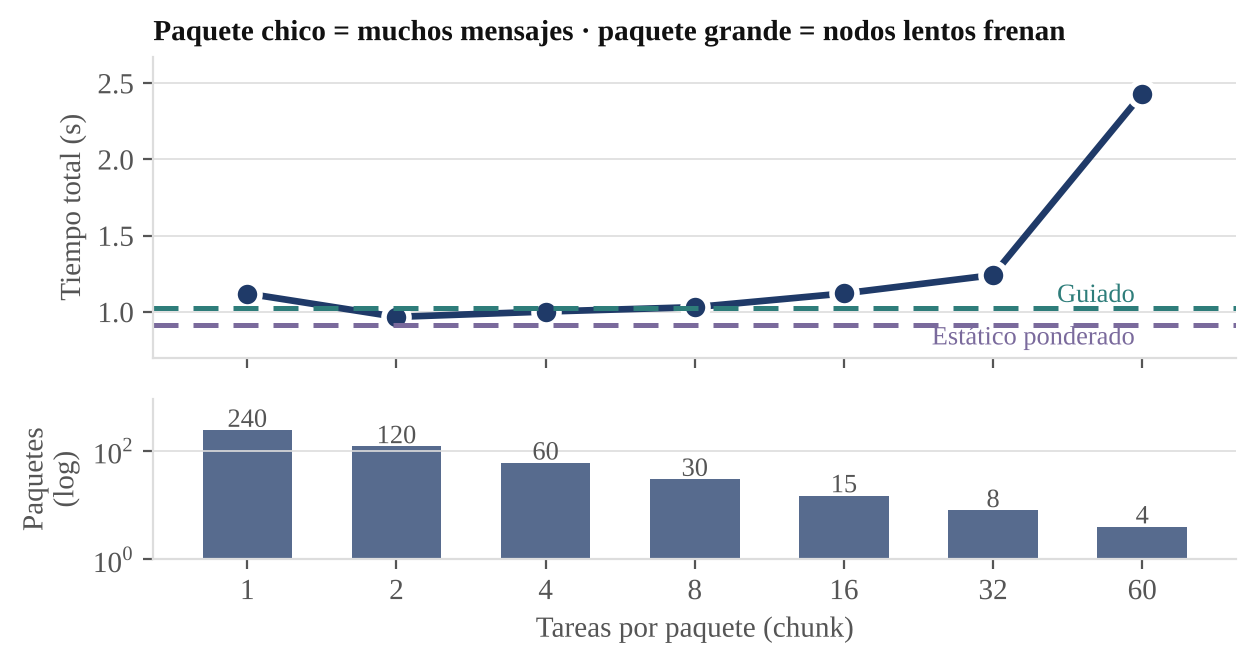
\includegraphics[width=\linewidth,height=3.6cm,keepaspectratio]{../resultados/figuras_formal/chunk.png}\\[4pt]
{\footnotesize mejor: \textbf{\color{dinamico}\chunkMejor} (\tChunkMejor\,s) \;·\; peor: \textbf{\color{estatico}\chunkPeor} (\tChunkPeor\,s)}
\column{.02\textwidth}
\column{.49\textwidth}\centering
{\etq{suave}{Escalabilidad: más nodos}}\\[2pt]\linea\\[4pt]
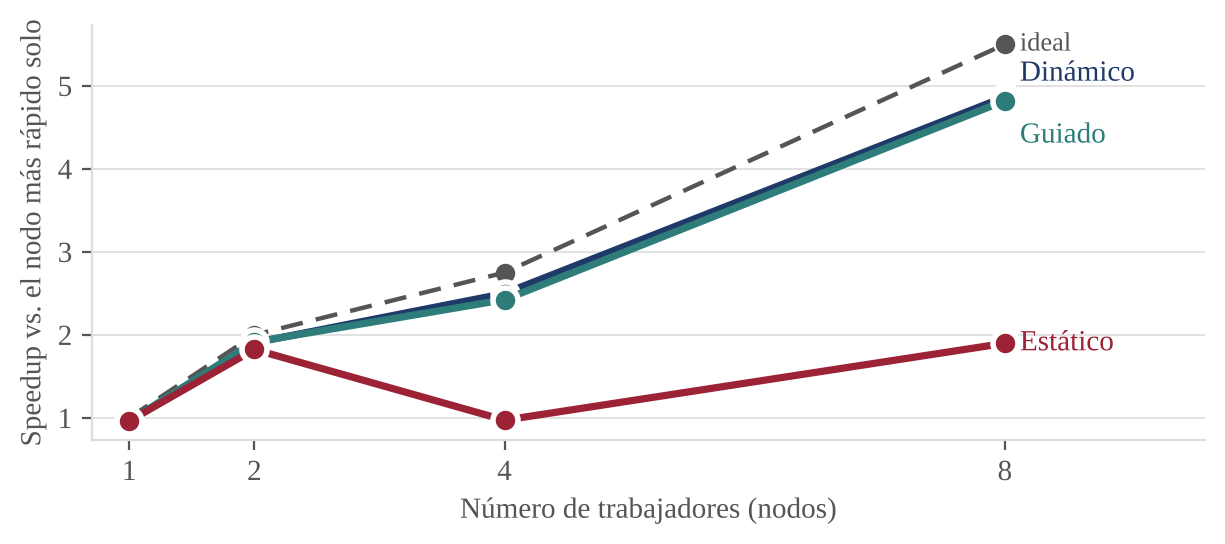
\includegraphics[width=\linewidth,height=3.6cm,keepaspectratio]{../resultados/figuras_formal/escalabilidad.png}\\[4pt]
{\footnotesize con 8 nodos: dinámico \textbf{\color{dinamico}\spDinOcho$\times$} \;·\; estático \textbf{\color{estatico}\spEstOcho$\times$}}
\end{columns}
\note[item]{Paquete: hay un compromiso. Muy chico genera muchos mensajes; muy grande deja a un nodo lento con demasiado trabajo. Con 60 tareas por paquete el tiempo se dispara a más de 2 segundos, igual de malo que el estático.}
\note[item]{El barrido usa una latencia simulada de 3\,ms por petición. Entre paquetes de 2 a 8 el tiempo casi empata; la diferencia es ruido de medición.}
\note[item]{Escalabilidad: speedup contra un nodo rápido trabajando solo. El estático casi no mejora porque lo frena el nodo más lento; con 8 trabajadores el dinámico logra \spDinOcho$\times$ y el estático solo \spEstOcho$\times$.}
\end{frame}

% ===================================================================== (nueva) clúster 1
\section{Clúster de laptops}
\begin{frame}[fragile]{Aplicación al clúster de laptops}
\begin{columns}[T,onlytextwidth]
\column{.55\textwidth}
\centering
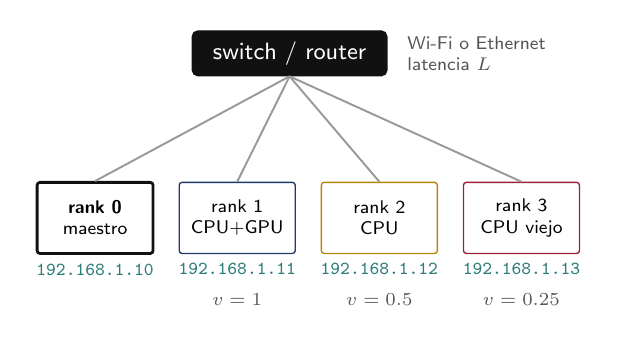
\begin{tikzpicture}[scale=.95,transform shape,
  lap/.style={rounded corners=1pt,draw=tinta,fill=hoja,line width=.5pt,minimum width=1.55cm,minimum height=.95cm,align=center,inner sep=2pt,font=\scriptsize}]
  \node[nodo,draw=tinta,fill=tinta,text=papel,minimum width=2.6cm] (sw) at (2.6,2.2) {\small switch / router};
  \node[lap,draw=tinta,line width=1pt] (m) at (0,0) {\textbf{rank 0}\\maestro};
  \node[lap,draw=dinamico] (a) at (1.9,0) {rank 1\\CPU+GPU};
  \node[lap,draw=ocre] (b) at (3.8,0) {rank 2\\CPU};
  \node[lap,draw=estatico] (c) at (5.7,0) {rank 3\\CPU viejo};
  \foreach \n in {m,a,b,c}{\draw[trazo,line width=.7pt] (sw.south) -- (\n.north);}
  \node[txtm,anchor=north] at (m.south) {192.168.1.10};
  \node[txtm,anchor=north] at (a.south) {192.168.1.11};
  \node[txtm,anchor=north] at (b.south) {192.168.1.12};
  \node[txtm,anchor=north] at (c.south) {192.168.1.13};
  \node[txtp,anchor=north] at ([yshift=-.4cm]a.south) {$v=1$};
  \node[txtp,anchor=north] at ([yshift=-.4cm]b.south) {$v=0.5$};
  \node[txtp,anchor=north] at ([yshift=-.4cm]c.south) {$v=0.25$};
  \node[txtp,anchor=west,align=left] at (4.05,2.2) {Wi-Fi o Ethernet\\latencia $L$};
\end{tikzpicture}\\[2pt]
{\fontsize{8.5}{10}\selectfont\color{suave}Direcciones IP y velocidades $v$: ejemplo ilustrativo.}
\column{.43\textwidth}
\begin{block}{Ejecución en el clúster}
\begin{lstlisting}[language={},basicstyle=\ttfamily\fontsize{6.4}{7.4}\selectfont,literate={}]
# hosts.txt   (IP:procesos)
192.168.1.10:1   # maestro
192.168.1.11:1
192.168.1.12:1
192.168.1.13:1

mpiexec -f hosts.txt -n 4 \
  python balanceo.py \
  --estrategia dinamico --chunk 8 \
  --modo real --velocidades 1
\end{lstlisting}
\end{block}
\vspace{2pt}
{\small Mismo código que la simulación: cambia solo \mono{mpiexec}.}
\end{columns}
\note[item]{Aplicación al clúster: cuatro laptops conectadas por la misma red local, a través de un switch o un router Wi-Fi. El rank 0 es el maestro y vive en una de las laptops; los otros tres ranks son trabajadores. Cada laptop se identifica por su dirección IP; las que aparecen aquí son de ejemplo.}
\note[item]{El archivo hosts.txt le dice a mpiexec en qué IP arrancar cada proceso. Cada laptop necesita la misma versión de Python, mpi4py y MPI, el proyecto en la misma ruta, y acceso por SSH sin contraseña desde el maestro (en Windows se usa MS-MPI). El diagnóstico se corre con cluster\_diagnostico.py.}
\note[item]{La heterogeneidad ahora es real: una laptop con GPU, una intermedia y una vieja. Con el modo real ya no se simulan velocidades; cada nodo tarda lo que su hardware le permita. El algoritmo dinámico no necesita saber cuál es cuál: el que termina antes pide antes.}
\end{frame}

% ===================================================================== (nueva) clúster 2
\begin{frame}{Latencia, paquete y balanceo CPU/GPU}
\begin{columns}[T,onlytextwidth]
\column{.5\textwidth}
{\etq{suave}{Un paquete en la red}}\\[2pt]\linea\\[3pt]
\centering

\begin{tikzpicture}[scale=.82,transform shape]
  \fill[estatico] (0,0) rectangle (.9,.5);
  \fill[ocre] (.9,0) rectangle (1.8,.5);
  \fill[dinamico] (1.8,0) rectangle (5.9,.5);
  \node[txtp,text=papel,font=\scriptsize\bfseries] at (.45,.25) {$L$};
  \node[txtp,text=papel,font=\scriptsize\bfseries] at (1.35,.25) {$L$};
  \node[text=papel,font=\scriptsize\bfseries] at (3.85,.25) {$k\,\bar c / v$};
  \node[txtm,anchor=north,text=estatico] at (.45,-.05) {PEDIR};
  \node[txtm,anchor=north,text=ocre] at (1.35,-.05) {TRABAJO};
  \node[txtp,anchor=north] at (3.85,-.05) {cómputo en el nodo};
\end{tikzpicture}\\[3pt]
\raggedright
\begin{block}{Sobrecosto de comunicación}
$f=\dfrac{2L}{2L+k\bar c/v}\le 0.1 \;\Rightarrow\; k\ge 18\,L\,v/\bar c$
\end{block}
\vspace{2pt}
{\small Ejemplo: $L=3$\,ms, $\bar c=10$\,ms, $v=1$ $\Rightarrow$ $k\ge 5.4$. Con mensajes de pocos bytes domina la \textbf{latencia}, no el ancho de banda.}
\column{.02\textwidth}
\column{.46\textwidth}
{\etq{suave}{CPU, GPU y velocidad relativa}}\\[2pt]\linea\\[4pt]
\small\renewcommand{\arraystretch}{1.02}\arrayrulecolor{regla}
\begin{tabular}{@{}l@{\hspace{.35cm}}l@{\hspace{.35cm}}l@{}}
\toprule[.6pt]
\etq{suave}{Nodo} & \etq{suave}{$v_i$} & \etq{suave}{Paquetes}\\ \midrule[.4pt]
CPU + GPU & 1 & \ok{más}\\
CPU actual & 0.5 & medio\\
CPU viejo & 0.25 & \ko{menos}\\
\bottomrule[.6pt]
\end{tabular}\\[5pt]
{\footnotesize $v_i=\text{rend}_i/\text{rend}_{\text{máx}}$, medido con \mono{cluster\_diagnostico.py}}\\[2pt]
\begin{exampleblock}{Qué balanceo usar}
{\footnotesize \textbf{Dinámico:} sin $v_i$ \;·\; \textbf{ponderado:} con $v_i$}
\end{exampleblock}
\end{columns}
\note[item]{Latencia. Cada paquete cuesta dos viajes por la red (PEDIR y TRABAJO), de L cada uno, antes de que el trabajador pueda calcular. Si las tareas son muy cortas, ese overhead domina y el cómputo útil se diluye.}
\note[item]{Fórmula: la fracción de sobrecosto f es dos veces L entre dos L más el cómputo del paquete, k por el costo medio entre la velocidad. Para mantener f por debajo de 10 \% se despeja k mayor o igual a 18 por L por v entre c barra. Con L de 3 ms, tareas de 10 ms y v igual a 1, k debe ser al menos 5.4. En la simulación casi no hay latencia (L cercana a cero), por eso paquetes chicos empatan; en una red real la cota sube y el paquete óptimo crece.}
\note[item]{Ancho de banda: los mensajes son listas de unos pocos enteros, es decir bytes; por eso lo que importa es la latencia y no el ancho de banda de la red. En Wi-Fi la latencia es mayor y más variable que en Ethernet, así que el paquete óptimo crece.}
\note[item]{CPU y GPU: la velocidad relativa v de cada nodo es su rendimiento (tareas por segundo) dividido entre el del más rápido; no importa si el trabajo lo hace una CPU o una GPU. Con balanceo dinámico no hace falta conocer v: la laptop con GPU pide paquetes más seguido. El estático ponderado sí necesita v medida y no reacciona si el nodo se degrada.}
\note[item]{El script cluster\_diagnostico.py mide por nodo la IP, el RTT al maestro, la velocidad relativa y si hay GPU, y sugiere el valor de --velocidades y el tamaño de paquete k.}
\end{frame}

% ===================================================================== 17
\section{Cierre}
\begin{frame}{Conclusiones y trabajo futuro}
\begin{columns}[T,onlytextwidth]
\column{.6\textwidth}
\renewcommand{\arraystretch}{1}\arrayrulecolor{regla}
\begin{tabular}{@{}>{\kalamL\fontsize{26}{28}\selectfont\color{estatico}}p{.9cm}p{7cm}@{}}
1 & \textbf{Estático:} simple y barato, pero un nodo lento frena a todos (\tEstHet\,s).\\[8pt]\midrule[.4pt]
2 & \textbf{Dinámico:} asigna paquetes a quien se desocupa, sin conocer velocidades (\tDinHet\,s).\\[8pt]\midrule[.4pt]
3 & \textbf{El paquete importa:} ni muy chico ni muy grande; el guiado no siempre gana (\tGuiHet\,s).
\end{tabular}
\column{.36\textwidth}
\begin{alertblock}{Limitaciones}
\begin{itemize}\setlength\itemsep{0pt}\footnotesize
\item Nodos simulados (\mono{sleep}), una laptop
\item Sin red física en los resultados
\item El maestro puede ser cuello de botella
\end{itemize}
\end{alertblock}
\vspace{2pt}
\begin{exampleblock}{Trabajo futuro}
\begin{itemize}\setlength\itemsep{0pt}\footnotesize
\item Prefetch con \mono{isend/irecv}
\item Robo de trabajo sin maestro
\item Medir en un clúster real
\end{itemize}
\end{exampleblock}
\end{columns}
\note[item]{Tres ideas para cerrar: estático simple pero frágil; dinámico se adapta; y el tamaño del paquete es la perilla importante (el guiado no siempre gana porque su primer paquete grande puede caer en el nodo lento).}
\note[item]{Regla práctica: si no conozco las velocidades o no son estables, dinámico. Si las conozco y las tareas son parejas, estático ponderado es más simple y barato.}
\note[item]{Sé honesto con las limitaciones: la simulación es una abstracción; en un cluster real habría red, memoria y contención.}
\end{frame}

% ===================================================================== 18
\begin{frame}{¿Preguntas? · Referencias}
\begin{columns}[T,onlytextwidth]
\column{.28\textwidth}
{\kalamL\fontsize{21}{24}\selectfont\color{tinta}¿Preguntas?}\\[6pt]
{\small\color{suave}Gracias por su atención}\\[10pt]
{\fontsize{8}{11}\selectfont\color{estatico}Jared Méndez Valencia\\Daniel del Valle Andrade\\Johan Lezama Núñez\\Camila Serrano Trinidad}
\column{.02\textwidth}
\column{.68\textwidth}
\fontsize{7.6}{9}\selectfont\setlength{\parindent}{-1.2em}\leftskip1.2em\raggedright
Dalcin, L., \& Fang, Y.-L. L. (2021). mpi4py: Status update after 12 years of development. \emph{Computing in Science \& Engineering, 23}(4), 47–54. \url{https://doi.org/10.1109/MCSE.2021.3083216}\par\vspace{3pt}
Fernandes, J. B., de Assis, Í. A. S., Martins, I. M. S., Barros, T., \& Xavier-de-Souza, S. (2024). \emph{Adaptive asynchronous work-stealing for distributed load-balancing in heterogeneous systems} [Preprint]. arXiv. \url{https://arxiv.org/abs/2401.04494}\par\vspace{3pt}
Message Passing Interface Forum. (2023). \emph{MPI: A message-passing interface standard, version 4.1}. \url{https://www.mpi-forum.org/docs/mpi-4.1/mpi41-report/mpi41-report.htm}\par\vspace{3pt}
OpenMP Architecture Review Board. (2021). \emph{OpenMP application programming interface, version 5.2}. \url{https://www.openmp.org/specifications/}\par\vspace{3pt}
Pacheco, P. S., \& Malensek, M. (2022). \emph{An introduction to parallel programming} (2nd ed.). Morgan Kaufmann.\par\vspace{3pt}
Rogowski, M., Aseeri, S., Keyes, D., \& Dalcin, L. (2023). mpi4py.futures: MPI-based asynchronous task execution for Python. \emph{IEEE Transactions on Parallel and Distributed Systems, 34}(2), 611–622.
\end{columns}
\note[item]{Todas las referencias son de 2021 en adelante, en formato APA 7.}
\note[item]{Preguntas frecuentes: ¿por qué sleep? (reproducible y sin depender de núcleos); ¿por qué el guiado fue peor? (primer paquete grande en el nodo lento); ¿qué pasa si el maestro falla? (trabajo futuro).}
\end{frame}

\end{document}
